\section{Experimental Evaluation}
\label{sec:exp}

{\bf Experimental environment.} All experiments in this section were
conducted on an 8-slave elastic cloud cluster using Linux Ubuntu 14.04
and Spark v1.4.  Each node had 4 cores and 16 GB of memory.  Spark
Standalone cluster manager and Hadoop 2.6 were used.

Because Spark is a lazy evaluation system, a \insql{materialize}
operation was appended to the end of each query, which consisted of
the count of nodes and edges.  In cases where the goal was to evaluate
a specific operation in isolation, we used warm start, which consisted
of materializing the graph upon load.  Each experiment was conducted 3
times, we report the average running time, which is representative
because we took great care to control variability.  Standard deviation
for each measure is at or below 5\% of the mean except in cases of
very small running times.

{\bf Data and evaluation methods.}  We evaluate performance of our
framework on two real open-source datasets:

\begin{enumerate}%[leftmargin=*]

\item DBLP\footnote{\url{dblp.uni-trier.de/xml}} contains
  co-authorship information from 1936 \linebreak through 2015, with over 1.5
  million author nodes and over 6 million undirected co-authorship
  edges.  Total data size: 250 MB.

\item nGrams\footnote{\url{storage.googleapis.com/books/ngrams/books/datasetsv2.html}}
  contains word co-occurrence information from 1520 through 2008, with
  over 1.5 million word nodes and over 65 million undirected
  co-occurrence edges.  Total data size: 40 GB.
\eat{
\item
  DELIS\footnote{\url{law.di.unimi.it/webdata/uk-union-2006-06-2007-05}}
  contains monthly snapshots of a portion of the Web graph focusing on
  the .uk domains from 05/2006 through 05/2007, with a total of over
  133 million nodes and over 5.5 billion directed edges\cite{BSVLTAG}.
  Data size: 1 TB.
}
\end{enumerate}

These datasets are not large by industry standards, but the nGrams set
is of comparable size to the LiveJournal dataset in~\cite{Xin2013} and
is commesurate with our cluster size.  These two datasets differ from
each other not only in size, but also in the evolutionary properties:
co-authorship network nodes have limited lifespan, while the nGrams
network grows over time and nodes persist for long durations.  All
figures in the body of this section are on the larger nGrams dataset.
Refer to the Appendix for the dblp figures.  We plan to carry out
further experiments with a larger
DELIS\footnote{\url{law.di.unimi.it/webdata/uk-union-2006-06-2007-05}}
dataset as we grow the cluster in the near future.

\subsection{Number of partitions}

\begin{figure*}[th!]
\centering
\begin{minipage}{3.3in}
  \centering
  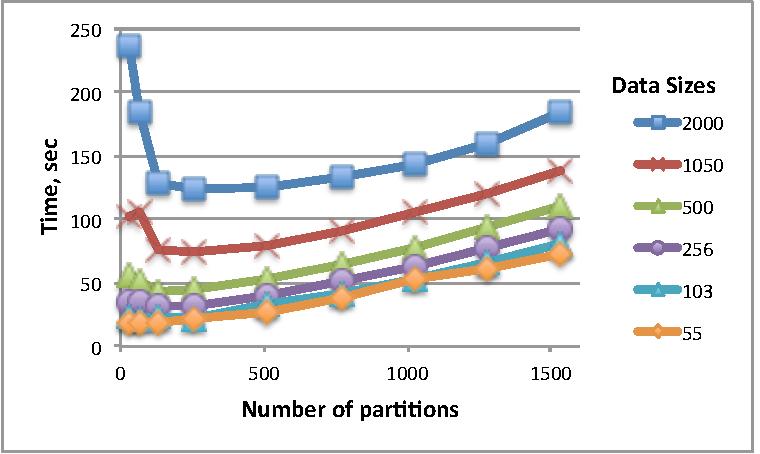
\includegraphics[width=3in]{figs/numparts.pdf}
  \caption{The number of partitions trend for different data sizes.}
  \label{fig:numparts}
\end{minipage}
\begin{minipage}{3.3in}
  \centering
  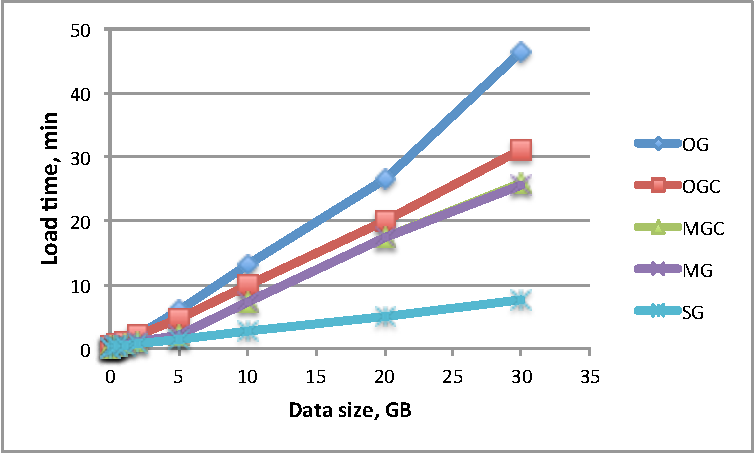
\includegraphics[width=3in]{figs/tselect.pdf}
  \caption{Total load time as a function of data size in the nGrams
    dataset.}
  \label{fig:tselect}
\end{minipage}
\end{figure*}

In Spark applications, one of the most influential performance drivers
is the choice of the number of partitions.  The default number of
partitions, based on the Hadoop block size, used to read the graphs in
practice proved insufficient.  We extended GraphX for parallel reading
of multiple files with a custom number of partitions.  For all
experiments a dynamic data size-based partition number estimator was
used based on the tuning experiment.

To tune the estimator, we ran a simple \insql{TSelect} query with each
data structure, varying the number of partitions on load for a range
of data sizes.  In each data structure, we observe the same trend --
as the number of partitions is increased for a given data size, the
system performance quickly improves, but then starts to deteriorate
(Figure~\ref{fig:numparts}).  This trend can be observed in all data
structures.  There is roughly a linear relationship between the data
size and the optimal number of partitions (see
Figure~\ref{fig:partsfit} in the Appendix), which allowed us to fit a
linear function and use it in all subsequent experiments.

\subsection{Data loading}

To understand how different data structures perform as a function of
data size, we ran a simple TSelect query:

\begin{small}
\begin{verbatim}
      TSelect V; E
      From    ngrams
      TWhere  Start >= x and End <= y
\end{verbatim}
\end{small}

\noindent where \insql{x} and \insql{y} parameters were varied to
achieve approximate desired data sizes for edge files.  Our file
format is a node file and an edge file per snapshot, with a node/edge
per line, respectively.  This format favors the SG data structure
because no data transformation, such as aggregation, is required.
This is substantiated experimentally, as can be seen in
Figure~\ref{fig:tselect}.  In the nGrams dataset, SG is the fastest
data structure for simple data loading, although all structures
exhibit a linear increase as a function of data size.  We observed the
same trend in both datasets and are not including the additional
graphs here. 

The significant influence of data format on data structure performance
has been shown previously~\cite{DBLP:journals/tos/MiaoHLWYZPCC15}.
Given the significant difference at size (3-5x) between SG and the
other data structures, an alternative file format for aggregated data
structures is warranted.  Because the load/materialize time varies so
significantly between different data structures, all subsequent
experiments are reported with a warm start, with application of a
desired partition strategy included during the loading process.

\subsection{\insql{TSelect} with \insql{TGroup}}

To investigate the comparative performance of different data
structures and partition strategies on the TGroup operation, we used
the following query:

\begin{small}
\begin{verbatim}
      TSelect Any V[vid, any(word)];
              Any E[vid1, vid2, sum(cnt) as score]
      From    nGrams
      TWhere  Start >= x And End <= y
      TGroup  by 8 years
\end{verbatim}
\end{small}

We kept the aggregation time window constant (8 years) and varied the
total number of snapshots in powers of 2.  Each snapshot contains
about 13 million edges.

Recollect that \insql{TGroup} requires a union and group by operation
in SG, combination of transform with filter and group by for MG, and
transform with filter for OG.  MGC, due its compactness, generally
outperforms MG and OGC -- OG, and here we include only the better
performing variant of each.  All data structures and partition
strategies show linear increase in Any-type aggregation time as the
number of snapshots grows.  As expected, because OGC is an already
aggregated data structure, it outperforms MGC and SG for the
\insql{TGroup} operation by two orders of magnitude in the largest
size.  This is shown in Figure~\ref{fig:tgroupe}, where we selected
only the fastest partition strategy for each data structure.  

\begin{figure*}[t!]
\centering
\begin{minipage}{3.3in}
  \centering
  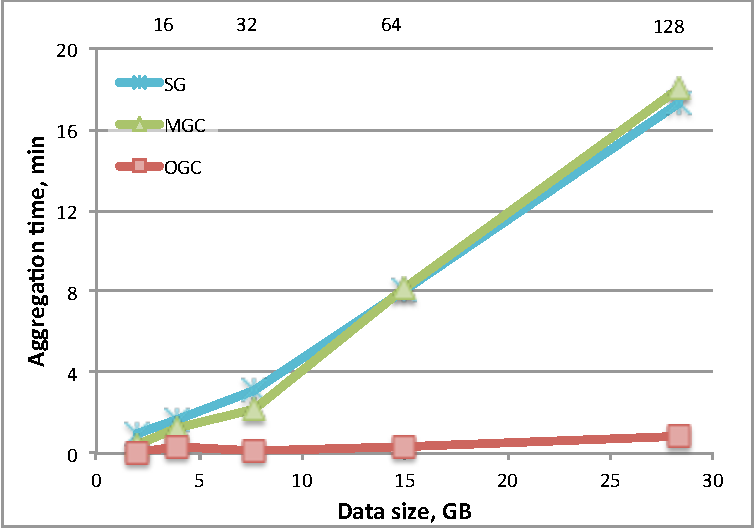
\includegraphics[width=3in]{figs/tgroupe_warm.pdf}
  \caption{\insql{TGroup} with Any after materialization.}
  \label{fig:tgroupe}
\end{minipage}
\begin{minipage}{3.3in}
  \centering
  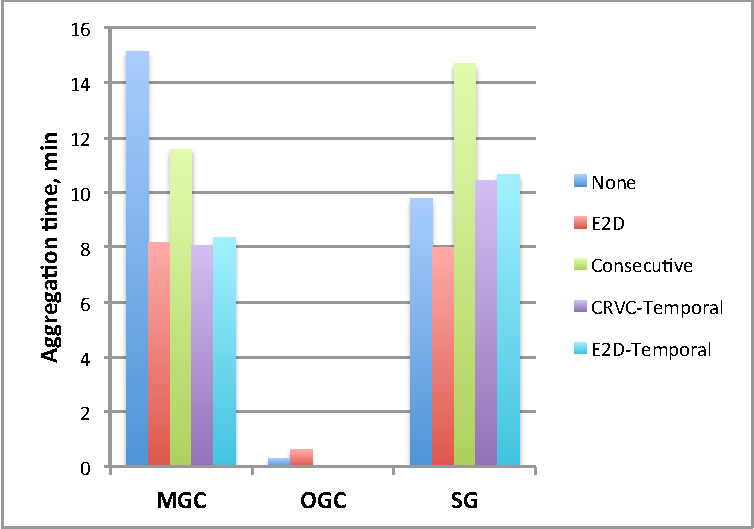
\includegraphics[width=3in]{figs/tgroupeparts.pdf}
  \caption{\insql{TGroup} by partition strategy.}
  \label{fig:tgroupeparts}
\end{minipage}
\end{figure*}

To compare between partition strategies, look at
Figure~\ref{fig:tgroupeparts}, which contains performance for each
data structure and strategy at 64 snapshot aggregation.  The same
pattern is observed at all aggregation sizes.  Partition strategies
can improve performance for the MGC data structure on this operation
-- all outperform the default partitioning case by 20\% or greater.
This can be explained by the group by operation that is performed on
the edges.  E2D always places two edges with the same key in the same
partition, which theoretically leads to least cross-partition
communication during aggregation.  Hybrid strategies use the
aggregation window as the width of the run, also placing the edges
that are to be grouped in the same set of partitions.  The difference
between E2D and the hybrid strategies for the MGC data structure are
not statistically significant.  E2D partitioning of the SG is also
beneficial, but the gains are smaller than for the MGC.  We observed
the same trend for the TGroup query with All semantics -- see
Appendix.

To demonstrate why we use warm start, consider
Figure~\ref{fig:tgroupe_cold}.  When we consider the total time for
the same query, including graph loading, partitioning, aggregation,
and materialization, the loading time dominates.  Based on this Figure
in isolation, where the fastest partition strategy per data structure
is depicted and is no partitioning, one can conclude that partitioning
is not beneficial (because it takes additional non-trivial time) and
that SG is the most effective data structure.  However, recall from
experiment 2 that the file format favors SG, and no conclusions should
be drawn from cold start total time alone.

OGC also outperforms the other data structures when we fix the overall
data size and vary the aggregation width, as can be seen in
Figure~\ref{fig:tgroupe_width}.  OGC performance is almost insensitive
to the aggregation width, with only a slight improvement as the width
increases.  SG and MGC show a linear increase, with a drop for the
final aggregation by the whole size.  This trend is observed in both
datasets -- see Appendix.

\begin{figure*}
\begin{minipage}{3.3in}
  \centering
  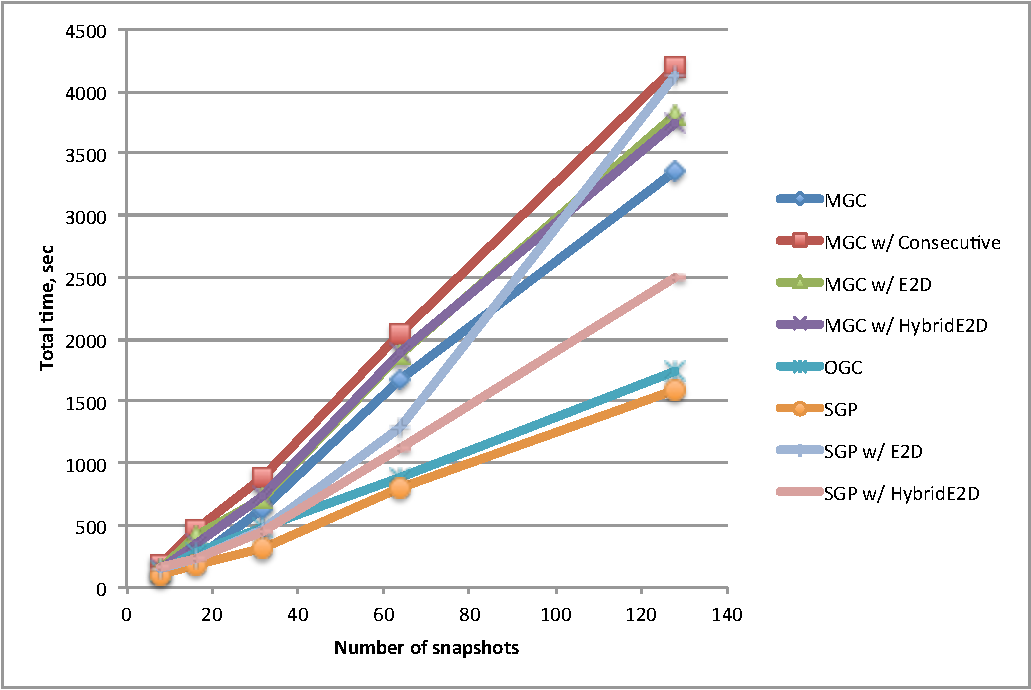
\includegraphics[width=3in]{figs/tgroupe_cold.pdf}
  \caption{\insql{TGroup} including materialization.}
\label{fig:tgroupe_cold}
\end{minipage}
\begin{minipage}{3.3in}
  \centering
  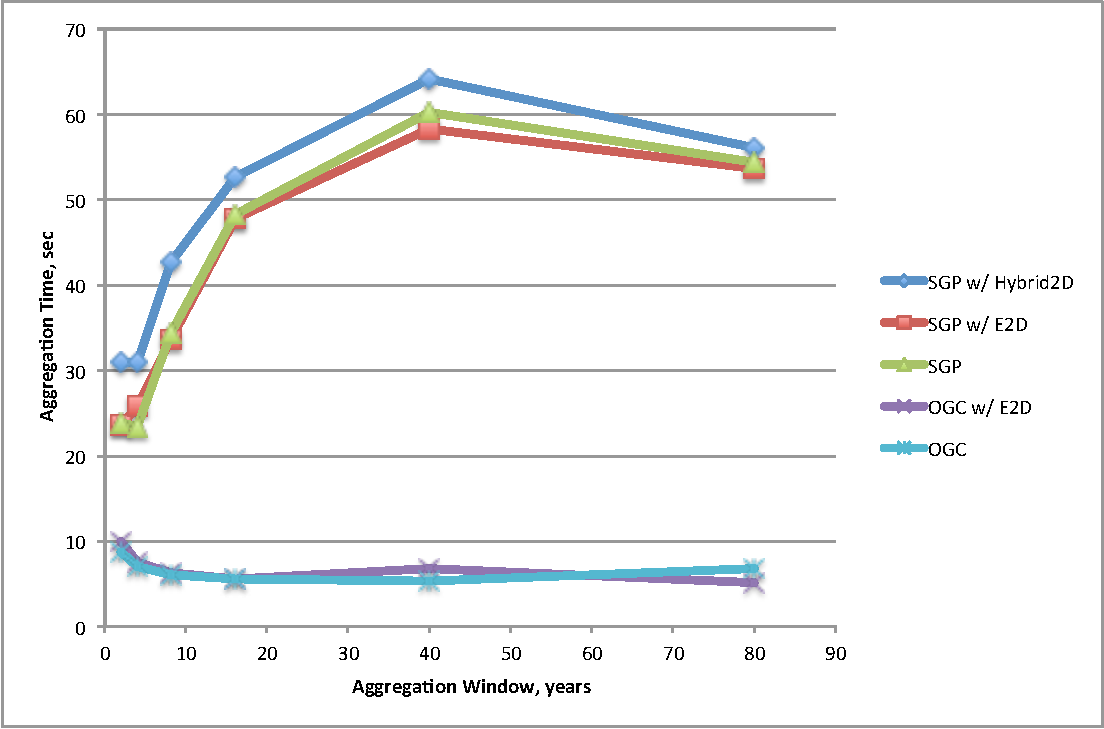
\includegraphics[width=3in]{figs/tgroupewidth.pdf}
  \caption{\insql{TGroup} with varying aggregation width.}
  \label{fig:tgroupe_width}
\end{minipage}
\end{figure*}

\subsection{\insql{TAnd} with \insql{All}}

\insql{TAnd} is a binary operation, and thus co-partitioning of the
two evolving graphs should play a role in performance.  Similarly to
\insql{TGroup} above, we look at the warm start performance of each
data structure and partition strategy, using the following query:

\begin{small}
\begin{verbatim}
      TSelect All V[vid, max(word)];
              All E[vid1, vid2, max(cnt) as score]
      From    ( TSelect V; E
                From nGrams
                TWhere  Start >= x And End <= y )
              TAnd
              ( TSelect V; E
                From nGrams
                TWhere  Start >= n And End <= m )      
\end{verbatim}
\end{small}

We are selecting the two graphs from the same dataset and varying the
amount of temporal overlap (\insql{n - m}) between them to investigate
the worst-case performance.  This query is a good example where query
optimization would lead to some performance improvement, since only
the \insql{n} to \insql{y} snapshots are relevant to the operation.
In this experiment the query was not optimized and was executed
directly as specified.

\insql{TAnd} requires a join operation for each snapshot pair in SG,
and a single graph join in all other data structures.  As the temporal
overlap between the two graphs increases, we expect OGC to outperform
SG for most cases, and this can be shown experimentally
(Figure~\ref{fig:tandall}).  SG performs well on the small temporal
overlap cases because fewer vertices and edges are joined there
compared to MGC/OGC.  Partitioning has a mild benefit for MGC,
especially with the E2D strategy, as it does for OGC and SG. See
Figure~\ref{fig:tand_parts} in the Appendix for side-by-side
comparison.

\begin{figure}[t!]
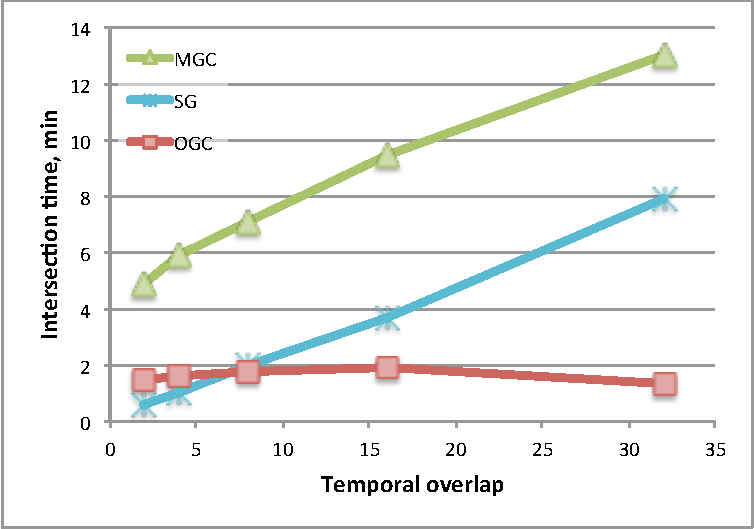
\includegraphics[width=3.2in]{figs/tand_all_warm.pdf}
\caption{\insql{TAnd} with varying temporal overlap.}
\label{fig:tandall}
\end{figure}

\insql{TOr} performance with \insql{Any} exactly matches that of
\insql{TAnd} with \insql{All} above where the snapshots are selected
from the same dataset, so we do not show it here.

\subsection{Pagerank}

Snapshot-based analytics like \insql{pagerank} are implemented using
the Pregel API in GraphX, with batch mode for MGC and OGC.  We used
the following query to evaluate data structure performance over
varying number of snapshots:

\begin{small}
\begin{verbatim}
      TSelect V[vid, pagerank()];
              E[vid1, vid2]
      From    nGrams
      TWhere  Start >= x And End <= y
\end{verbatim}
\end{small}

PageRank was executed for 10 iterations or until convergence,
whichever came first.  Performance of Pregel-based algorithms depends
heavily on the partition strategy, with best results achieved where
cross-partition communication is small.  For this reason, we evaluated
only no partitioning and Edge 2D partition strategy.

SG performs better than the other data structures in this experiment,
contrary to our expectation that the batch mode of MGC and OGC would
be faster (Figure~\ref{fig:pagerank}.  This can be explained by MGC
and OGC using significantly more cross-partition communication due to
the following factors:

\begin{enumerate}[leftmargin=*]
\item Each individual snapshot is less dense than the aggregate
  (although this depends on the rate of change, etc.) and dense graphs
  do worse with Pregel analytics.
\item Individual snapshots are smaller and take fewer partitions, so
  less communication happens cross-partition.
\item Pagerank gets faster as vertex values stabilize because those
  vertices stop sending out new messages. With each vertex sending a
  message for all snapshots where it exists at the same time, it takes
  as long to stop sending as the longest snapshot.  
\item The messages themselves for OGC are larger - it is more costly
  to send a Map object than a simple number.
\end{enumerate}

\begin{figure}[t]
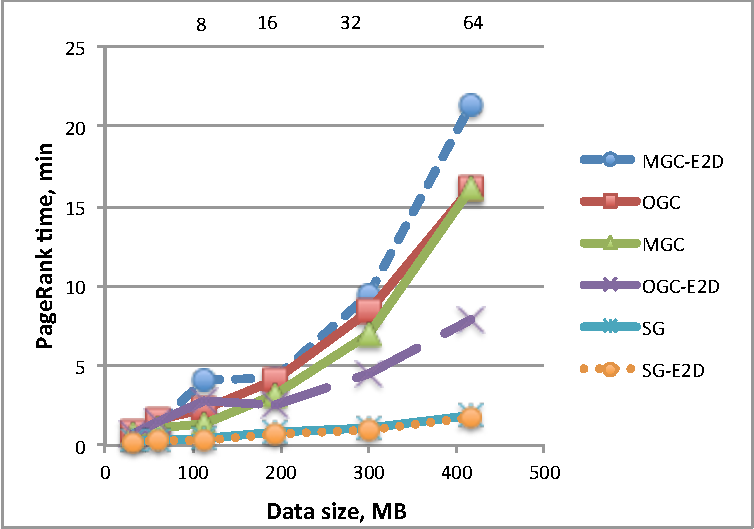
\includegraphics[width=3.2in]{figs/pagerank.pdf}
\caption{Pagerank performance over nGrams dataset.}
\label{fig:pagerank}
\end{figure}

As expected, E2D partitioning leads to performance improvements in all
data structures except MGC.

\subsection{\insql{TSelect} with \insql{trend(pagerank())}}

All the experiments above evaluated performance of single operations.
To see how data structures compare overall, we executed the following
query:

\begin{small}
\begin{verbatim}
      Select vid, pr
      From (TSelect Any V[vid, trend(prank) as pr]
                    Any E
            From (TSelect All V[vid, pagerank() as prank]; 
                          All E
                  From nGrams
                  TWhere Start >= x And End <= y
                  TGroup by 8 years)
            TGroup by size).toVerticesFlat
      Order by pr
      Limit 10
\end{verbatim}
\end{small}

As we saw above, typically SG loads faster and performs pagerank
faster, while OGC is very efficient at aggregation, and this query
combines all of these and adds trend analytics and projection into a
flat vertex relation for sort and limit.  The two data structures
perform comparably with the best partition strategy (E2D for OGC, none
for SG), as can be seen in Figure~\ref{fig:complexq}.

\begin{figure}[t]
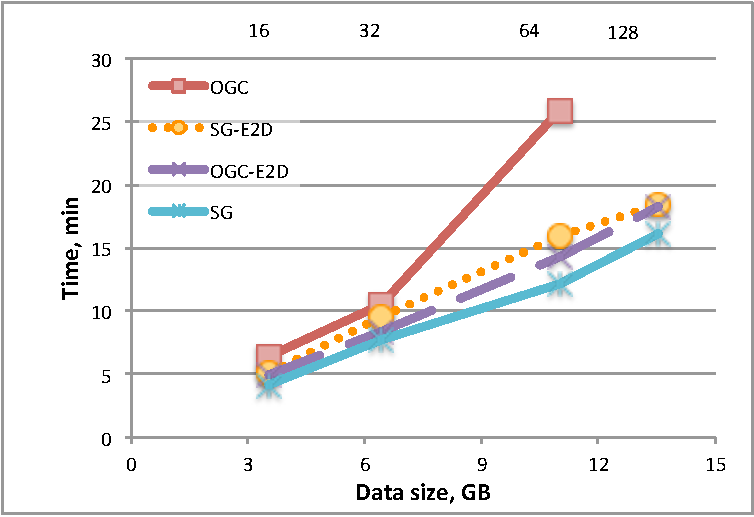
\includegraphics[width=3.2in]{figs/complexq.pdf}
\caption{Complex query with aggregation, pagerank, and trend over
  nGrams dataset.}
\label{fig:complexq}
\end{figure}

\vera{SOME CONCLUDING SENTENCE HERE}
